\documentclass[a4paper,twoside]{report}

\usepackage{geometry}
\usepackage{multicol}
\usepackage{caption}
\usepackage{graphicx}
\usepackage{pgf}
\usepackage{multirow}
\usepackage{wrapfig}
\usepackage{indentfirst}
\usepackage{setspace}
\usepackage{amsmath}
\usepackage{mathtools}

\geometry{
	top=2cm,
	bottom=2cm,
	left=2cm,
	right=2cm,
}
\graphicspath{{./img/}}
\setlength{\columnseprule}{1pt}

\newenvironment{Figure}
  {\par\medskip\minipage{\linewidth}}
  {\endminipage\par\medskip}

\begin{document}
    {\large Lab 7: Transient Responses of Second-Order RLC Circuits }
    \hfill
    {\large \textbf{Pre-Lab 03-C-07} \par}
	\vspace{0.1in}
    {\large AmirHossein Habibvand - 810196447}
    \hfill
    \today \par
    {\large Nima Modares Gorji - 810196558 \par}
	\vspace{0.5in}

    \section*{Part 1}
        \subsection*{Series Circuit:}
        {
            \setstretch{1.5}
            For every RLC series circuit we have this equation:
            \begin{center}
                $\frac{d^2 V_c}{d t^2} + \frac{R}{L}\frac{d V_c}{d t} + \frac{1}{LC}V_c = \frac{1}{LC}V_s$
            \end{center}
            The particular solution is
            \begin{center}
                $V_{c_p} = V_s$
            \end{center}
            And the homogeneous solution satisfies the equation
            \begin{center}
                $\frac{d^2 I_{L_h}V_{c_h}}{d t^2} + \frac{R}{L}\frac{d V_{c_h}}{d t} + \frac{1}{LC} = 0$
            \end{center}
            By defining
            \begin{center}
                $\alpha = \frac{R}{2L}$ ,
                $\omega = \frac{1}{\sqrt{LC}}$
            \end{center}
            We can obtain the characteristic equation as
            \begin{center}
                $s^2 + 2\alpha s + \omega ^ 2 = 0$
            \end{center}
            The roots of the characteristic equation are
            \begin{center}
                $s_1 = -\alpha + \sqrt{\alpha ^ 2 - \omega ^ 2}$ ,
                $s_2 = -\alpha - \sqrt{\alpha ^ 2 - \omega ^ 2}$
            \end{center}
            And the homogeneous solution becomes
            \begin{center}
                $V_{c_h} = A_1e^{s_1t} + A_2e^{s_2t}$
            \end{center}
            The total solution now becomes
            \begin{center}
                $V_c = V_s + A_1e^{s_1t} + A_2e^{s_2t}$
            \end{center}
            The form of the roots s1 and s2 depend on the values of
            $\alpha$ and $\omega$. The following three cases are possible:
            \begin{enumerate}
                \item
                    $\alpha = \omega$: \textbf{Critically Damped System} \\
                    $s_1$ and $s_2$ are equal and real numbers: no oscillatory behavior.

                \item
                    $\alpha > \omega$: \textbf{Over Damped System} \\
                    $s_1$ and $s_2$ are real numbers but not equal: no oscillatory behavior.

                \item
                    $\alpha < \omega$: \textbf{Oscillatory Damped System} \\
                    $s_1$ and $s_2$ are complex numbers: system exhibits oscillatory behavior.

                \item
                    $\alpha = 0$: \textbf{Undamped System}

            \end{enumerate}
        }

        \subsection*{Parallel Circuit:}
        {
            \setstretch{1.5}
            For every RLC parallel circuit we have this equation:
            \begin{center}
                $\frac{d^2 I_L}{d t^2} + \frac{1}{RC}\frac{d I_L}{d t} + \frac{1}{LC}I_L = \frac{1}{LC}I_s$
            \end{center}
            The particular solution is
            \begin{center}
                $I_{L_p} = I_s$
            \end{center}
            And the homogeneous solution satisfies the equation
            \begin{center}
                $\frac{d^2 I_{L_h}}{d t^2} + \frac{1}{RC}\frac{d I_{L_h}}{d t} + \frac{1}{LC}I_{L_h} = 0$
            \end{center}
            By defining
            \begin{center}
                $\alpha = \frac{1}{2RC}$ ,
                $\omega = \frac{1}{\sqrt{LC}}$
            \end{center}
            We can obtain the characteristic equation as
            \begin{center}
                $s^2 + 2\alpha s + \omega ^ 2 = 0$
            \end{center}
            The roots of the characteristic equation are
            \begin{center}
                $s_1 = -\alpha + \sqrt{\alpha ^ 2 - \omega ^ 2}$ ,
                $s_2 = -\alpha - \sqrt{\alpha ^ 2 - \omega ^ 2}$
            \end{center}
            And the homogeneous solution becomes
            \begin{center}
                $I_{L_h} = A_1e^{s_1t} + A_2e^{s_2t}$
            \end{center}
            The total solution now becomes
            \begin{center}
                $I_L = I_s + A_1e^{s_1t} + A_2e^{s_2t}$
            \end{center}
            The form of the roots s1 and s2 depend on the values of
            $\alpha$ and $\omega$. The following three cases are possible:
            \begin{enumerate}
                \item
                    $\alpha = \omega$: \textbf{Critically Damped System} \\
                    $s_1$ and $s_2$ are equal and real numbers: no oscillatory behavior.

                \item
                    $\alpha > \omega$: \textbf{Over Damped System} \\
                    $s_1$ and $s_2$ are real numbers but not equal: no oscillatory behavior.

                \item
                    $\alpha < \omega$: \textbf{Oscillatory Damped System} \\
                    $s_1$ and $s_2$ are complex numbers: system exhibits oscillatory behavior.
            \end{enumerate}
        }


    \section*{Part 2}
        \subsection*{Critical resistance}
            in series circuits: $R_c = 2 \sqrt{\frac{L}{C}}$ ,
            in parallel circuits: $R_c = \frac{1}{2} \sqrt{\frac{L}{C}}$

        \subsection*{Resonant frequency}
            in series and parallel circuits: $\omega = \frac{1}{\sqrt{LC}}$
        \pagebreak
        \subsection*{Damping Factor}
            \begin{multicols}{2}\setlength{\columnseprule}{0pt}
                in series circuits: $\alpha = \frac{R}{2L}$

                in parallel circuits: $\alpha = \frac{1}{2RC}$
                \vfill\null
                \columnbreak
                \begin{Figure}
                    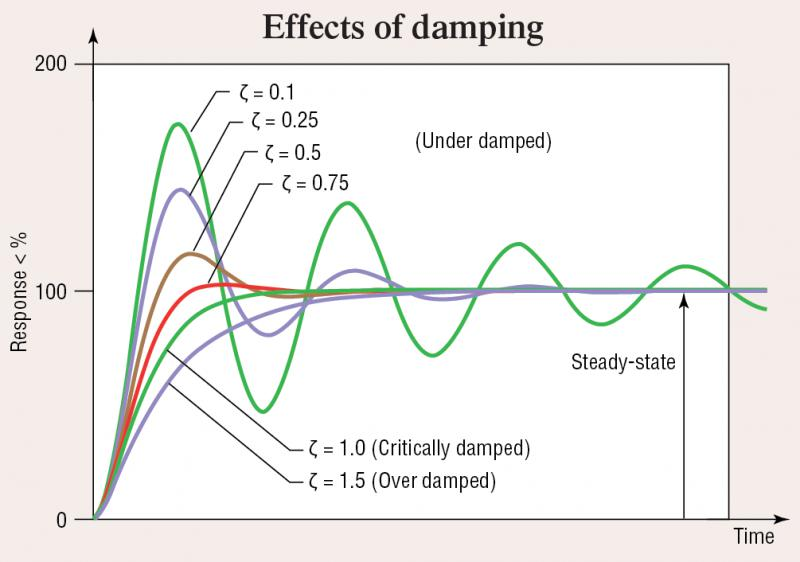
\includegraphics[width=0.8\textwidth]{damping.jpg}
                \end{Figure}
            \end{multicols}

        \subsection*{Overshoot}

    \section*{Part 3}
    {
        \setstretch{1.5}
        \begin{multicols}{2}\setlength{\columnseprule}{0pt}
            \subsection*{Series Circuit:}
                $
                    \left.
                    \begin{array}{l}
                        C = 3.3nF \\
                        L = 18mH \\
                        R = 1k\Omega \\
                        R_c = 2 \sqrt{\frac{L}{C}} \\
                        \omega = \frac{1}{\sqrt{LC}} \\
                    \end{array}
                    \right\}
                    \Longrightarrow
                    \left.
                        \begin{array}{l}
                            R_c = 4.6k\Omega \\
                            \omega = 129.8 kHz
                        \end{array}
                    \right.
                $
            \vfill\null
            \columnbreak
            \subsection*{Parallel Circuit:}
                $
                    \left.
                    \begin{array}{l}
                        C = 3.3nF \\
                        L = 18mH \\
                        R = 3k\Omega \\
                        R_c = \frac{1}{2} \sqrt{\frac{L}{C}} \\
                        \omega = \frac{1}{\sqrt{LC}} \\
                    \end{array}
                    \right\}
                    \Longrightarrow
                    \left.
                        \begin{array}{l}
                            R_c = 1.1k\Omega \\
                            \omega = 129.8 kHz
                        \end{array}
                    \right.
                $
        \end{multicols}
    }

    \section*{Part 4}
    {
        \setstretch{1.5}
        \begin{multicols}{2}\setlength{\columnseprule}{0pt}
            \subsection*{Series Circuit:}
                $
                    \left.
                    \begin{array}{l}
                        \tau = \frac{2L}{R} \\
                        L = 18mH \\
                        R = 1k\Omega \\
                    \end{array}
                    \right\}
                    \Longrightarrow
                    \tau = {36 * 10^{-6}}_{1/s}
                $
            \vfill\null
            \columnbreak
            \subsection*{Parallel Circuit:}
                $
                    \left.
                    \begin{array}{l}
                        \tau = 2RC \\
                        C = 3.3nF \\
                        R = 3k\Omega \\
                    \end{array}
                    \right\}
                    \Longrightarrow
                    \tau = {9.9 * 10^{-6}}_{1/s}
                $
        \end{multicols}
    }

    \section*{Part 5}

    \section*{Part 6}\setlength{\parindent}{0pt}.
        \begin{multicols}{2}\setlength{\columnseprule}{0pt}
            \subsection*{Resistor:}
                    $R = 0\Omega$ : Undamped System \\
                    $R = 3000\Omega$ : Oscillatory Damped System \\
                    $R = 4671\Omega$ : Critically Damped System \\
                    $R = 5500\Omega$ : Over Damped System
                \vfill\null
                \columnbreak
                \begin{center}
                    \begin{Figure}
                        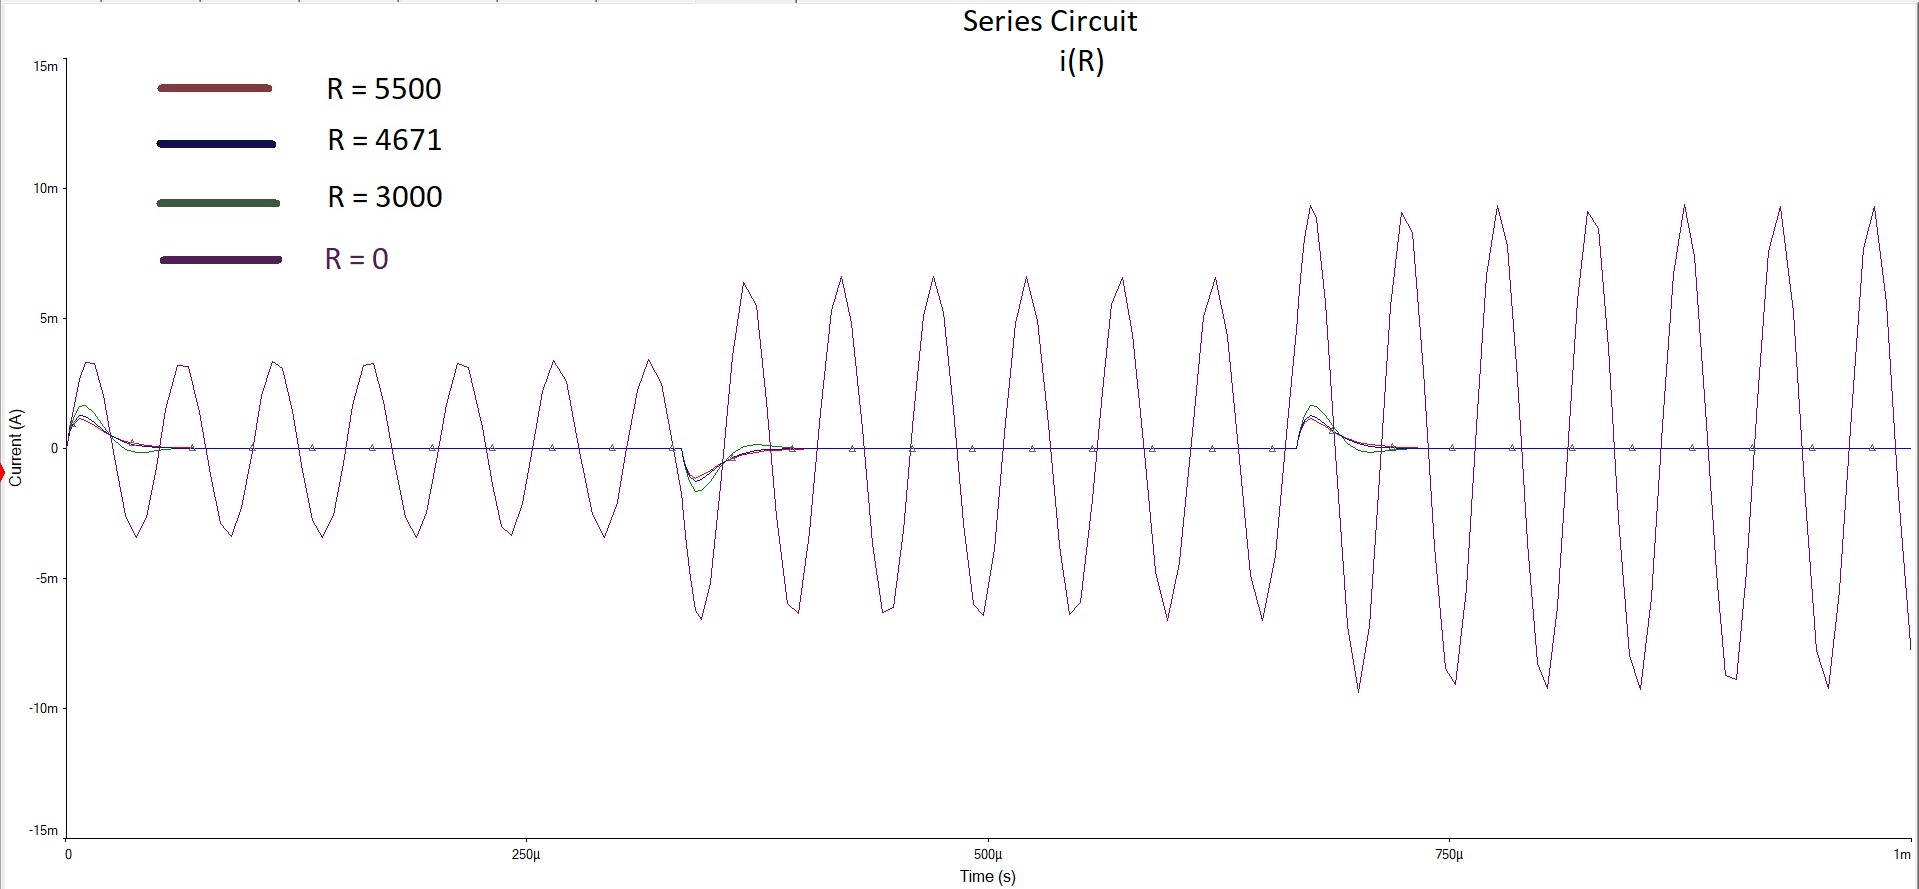
\includegraphics[width=\linewidth]{part6-resistor.jpg}
                    \end{Figure}
                \end{center}
        \end{multicols}
        \pagebreak
        \begin{multicols}{2}\setlength{\columnseprule}{0pt}
            \subsection*{Capacitor:}
                \vfill\null
                \columnbreak
                \begin{center}
                    \begin{Figure}
                        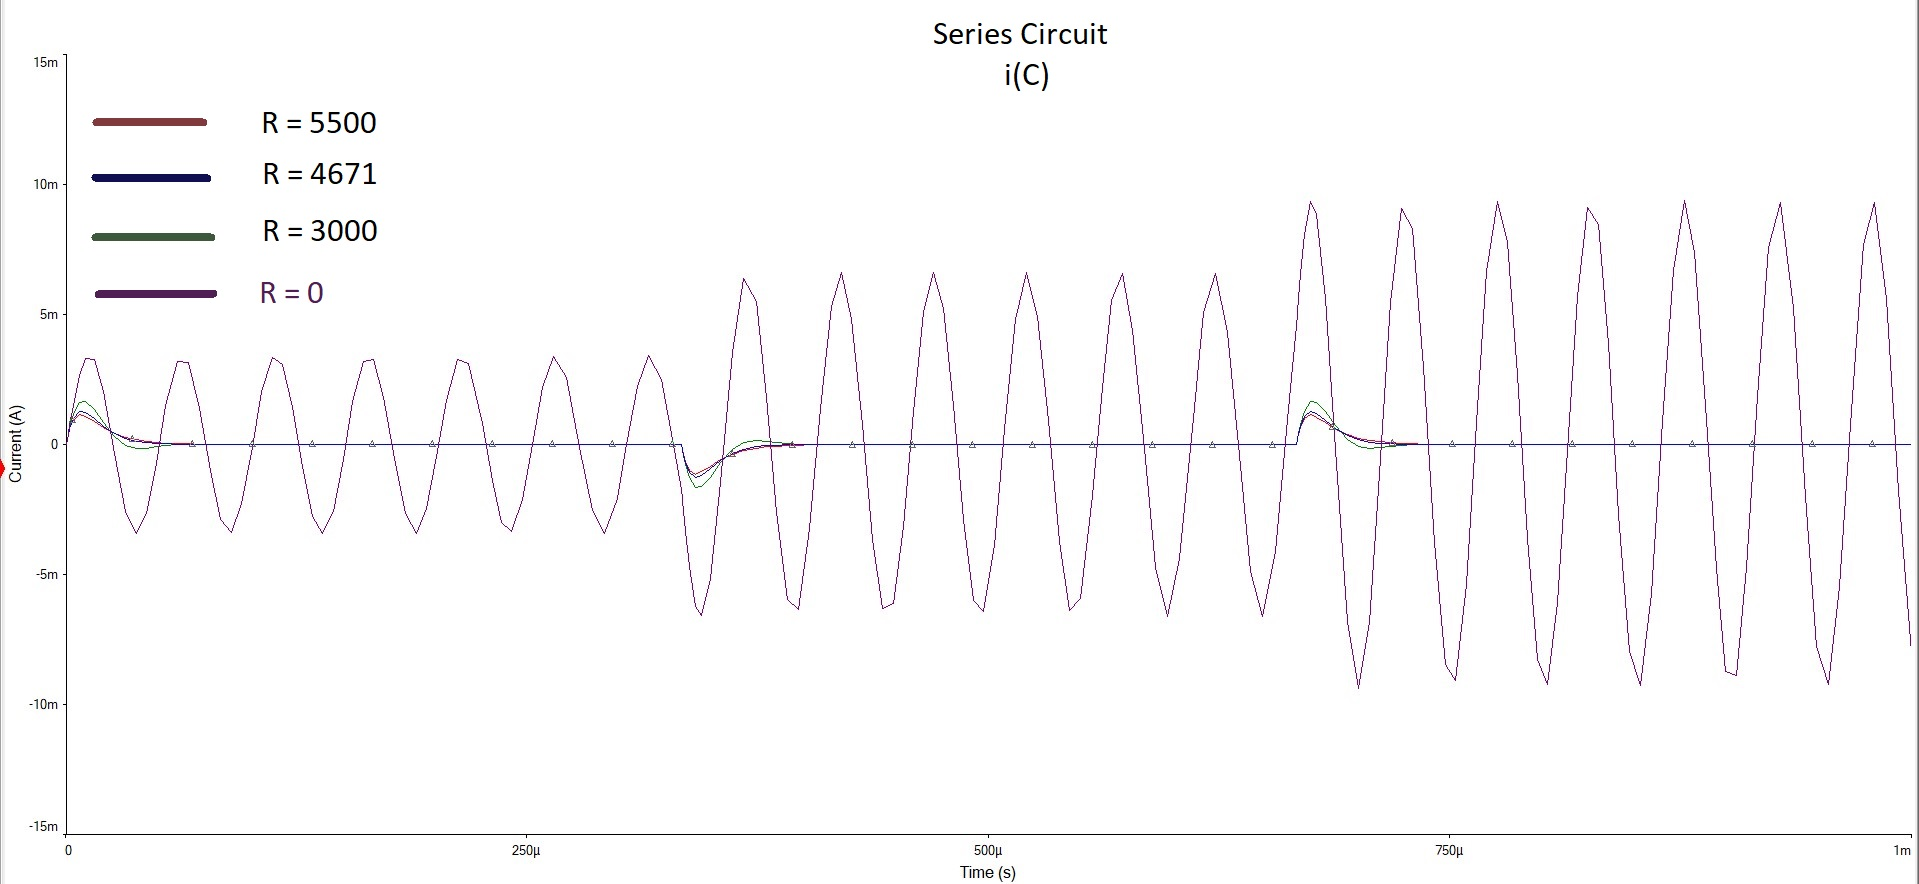
\includegraphics[width=\linewidth]{part6-capacitor.jpg}
                    \end{Figure}
                \end{center}
        \end{multicols}

        \begin{multicols}{2}\setlength{\columnseprule}{0pt}
            \subsection*{Inductor:}
                \vfill\null
                \columnbreak
                \begin{center}
                    \begin{Figure}
                        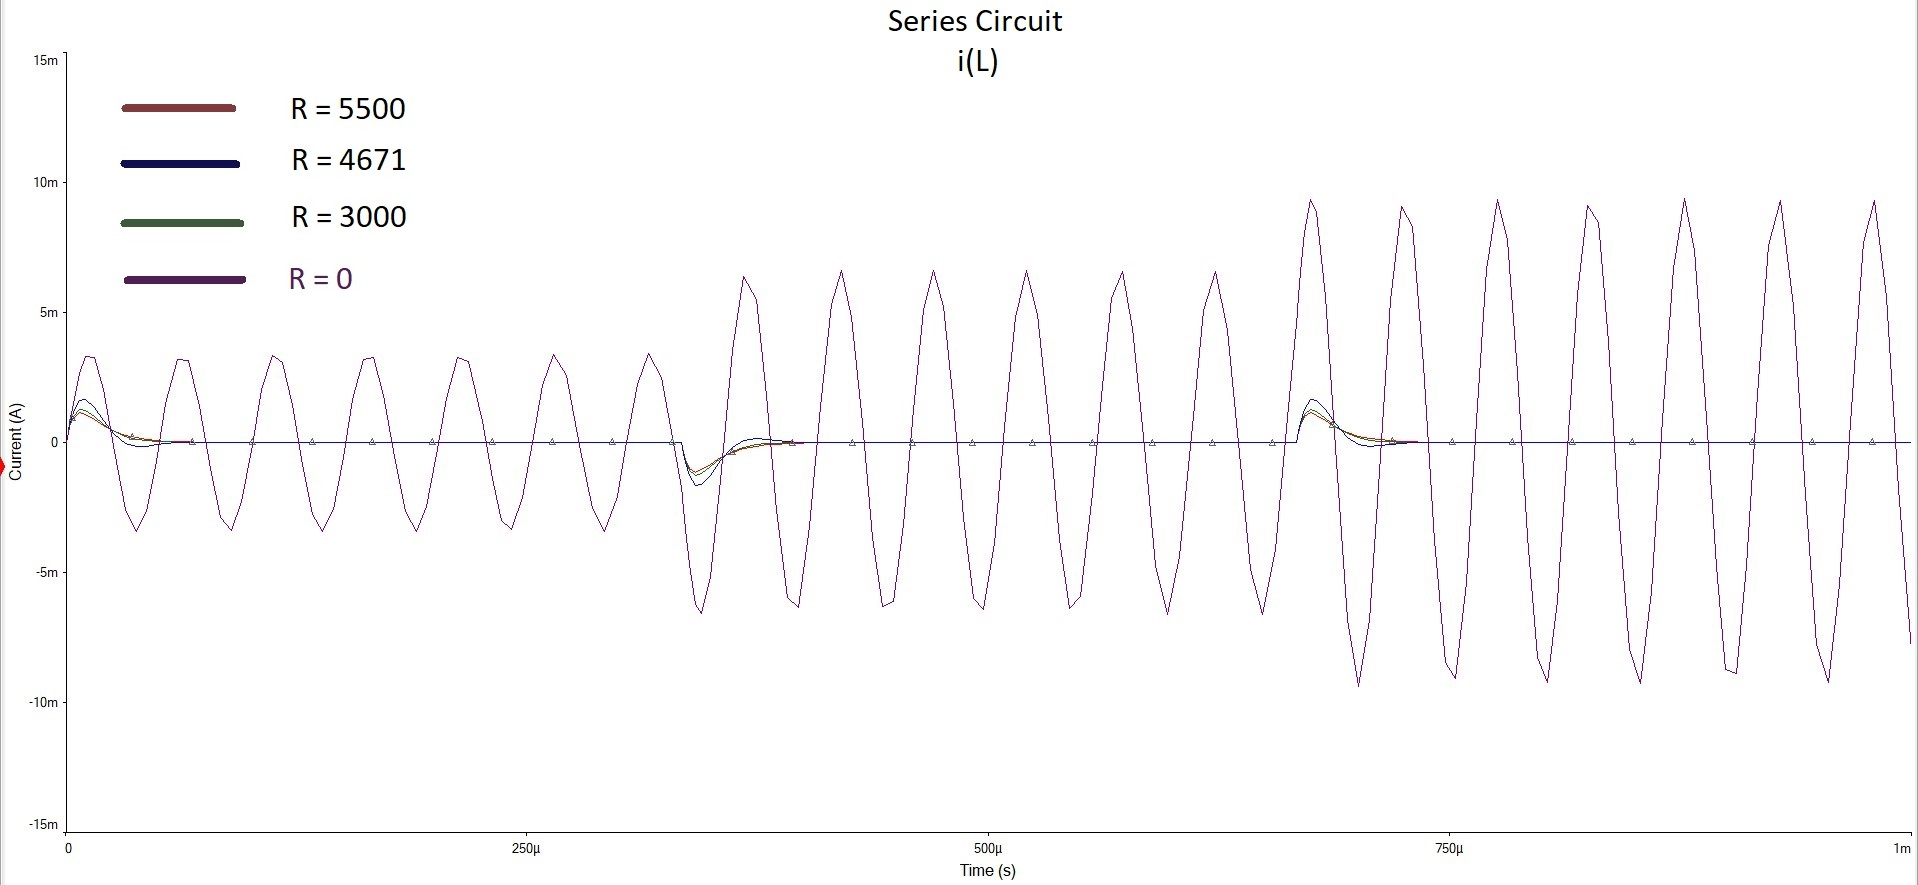
\includegraphics[width=\linewidth]{part6-inductor.jpg}
                    \end{Figure}
                \end{center}
        \end{multicols}
\end{document}
